\chapter{Software}
El software es el elemento lógico que forma parte del ordenador, todo aquello que es “intangible”. Es el \textbf{conjunto de programas y datos} que permiten manejar el \hyperlink{hardware}{hardware}, controlando y coordinando su funcionamiento para que realice las tareas deseadas.

% para no copiar un trozo que ya tenemos en el fichero 1_introduccion.tex

\ExecuteMetaData[1_introduccion]{tipossoftware}


\section{Licencias de Software}
A la hora de utilizar cualquier tipo de software lo habitual es que tengamos que aceptar una licencia, que es un contrato entre el licenciante (autor o titular de los derechos de explotación y/o distribución del software) y el licenciatario (el usuario o consumidor final).

Las licencias incluyen una serie de términos y condiciones, que son un conjunto de permisos que el autor otorga al usuario. Algunos ejemplos de condiciones en una licencia pueden ser:

\begin{itemize}
    \item Definir el tipo de uso.
    \item Limitar/permitir la distribución del software.
    \item Plazo de cesión de los derechos.
    \item Limitar/permitir la modificación del software.
\end{itemize}

Podemos representar los tipos de licencias a través de la siguiente imagen (Origen: {\href{https://en.wikipedia.org/wiki/Free_software\#Definition_and_the_Four_Essential_Freedoms_of_Free_Software}{Wikipedia}):

\begin{center}
    \vspace{-10pt}
    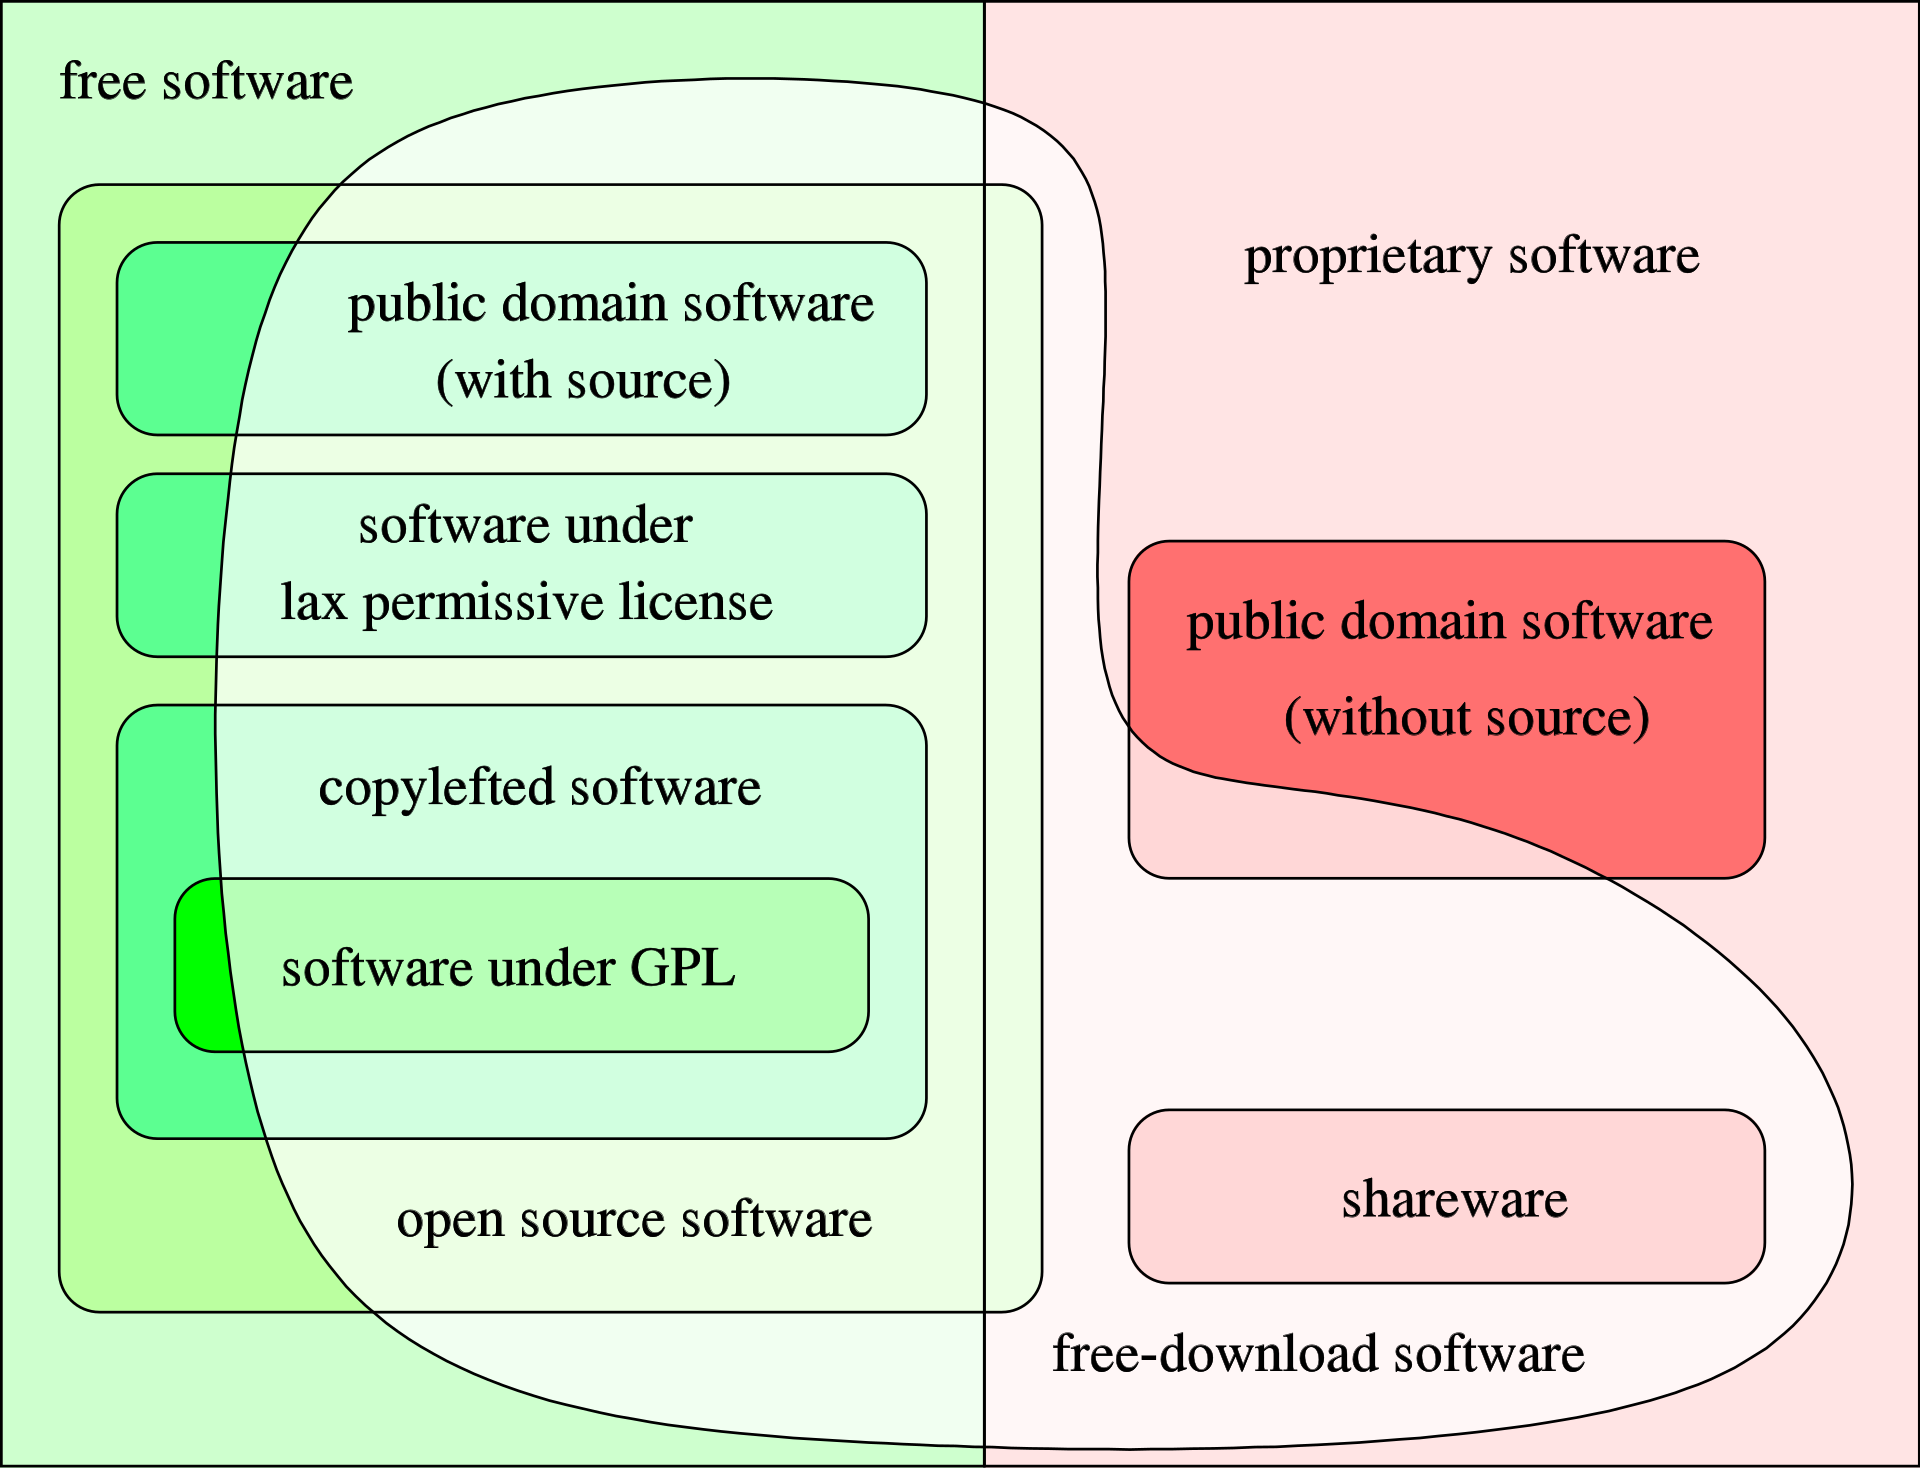
\includegraphics[width=0.65\linewidth]{free_and_nonfree_software.png}
\end{center}

% INCLUDE de sección de licencias libres
% modifico automáticamente secciones en subsecciones, y subsecciones en subsubsecciones

\let\foo\section %creo comando intermedio para luego recuperar cómo era la sección
\let\section\subsection
\let\subsection\subsubsection
% cambio el path de las imágenes
\graphicspath{{../../../temas_comunes/gnu_linux/img}}

\ExecuteMetaData[../../../temas_comunes/gnu_linux/gnu_linux]{softwarelibre}

%deshago todo lo hecho para la sección
\let\subsubsection\subsection
\let\subsection\section
\let\section\foo



\graphicspath{{img/si}}

% /INCLUDE

\subsection{Software privativo}
En contraposición al Software Libre se encuentra el software privativo, el cuál \textbf{no permite} el acceso al código fuente, ya que sólo se encuentra a disposición de los desarrolladores, no permitiendo su libre modificación, adaptación o distribución.

Dentro de este tipo de software podemos encontrar algunos tipos de licenciamiento conocidos:

\begin{itemize}
    \item \textbf{Freeware}: Normalmente se utiliza para el software que es gratuito pero que no permite la modificación del mismo.
    \item \textbf{Shareware}: El usuario puede evaluar de forma gratuita el producto, durante un tiempo limitado o con una funcionalidad limitada.
\end{itemize}

Entre el software más utilizado que es software privativo nos podemos encontrar a: Windows, Photoshop, juegos comerciales, ...

\subsection{Software de dominio público}
Es aquel que el autor decide publicarlo bajo el denominado \href{https://es.wikipedia.org/wiki/Dominio_p%C3%BAblico}{dominio público}, lo que hace que cualquiera pueda acceder al código fuente, modificarlo \textbf{pero también publicarlo bajo una licencia no libre}.

Este tipo de licencia suele ser aplicada a libros y música, por ejemplo, tras 70 años después de la muerte del autor.



%\section{Sistemas Operativos}
%
%El Sistema Operativo (\textbf{SO}) es el software que controla el hardware del ordenador, creando recursos lógicos y servicios que otro software y los usuarios pueden utilizar.














%    \section{Tipos de Software}
%    \subsection{firmware,sistema y aplicaciones}
%
%
%